\section{Demonstration}

\subsection{Interface Overview}

\begin{frame}{Interface Overview}
  \begin{figure}
    \begin{annotatedFigure}
      {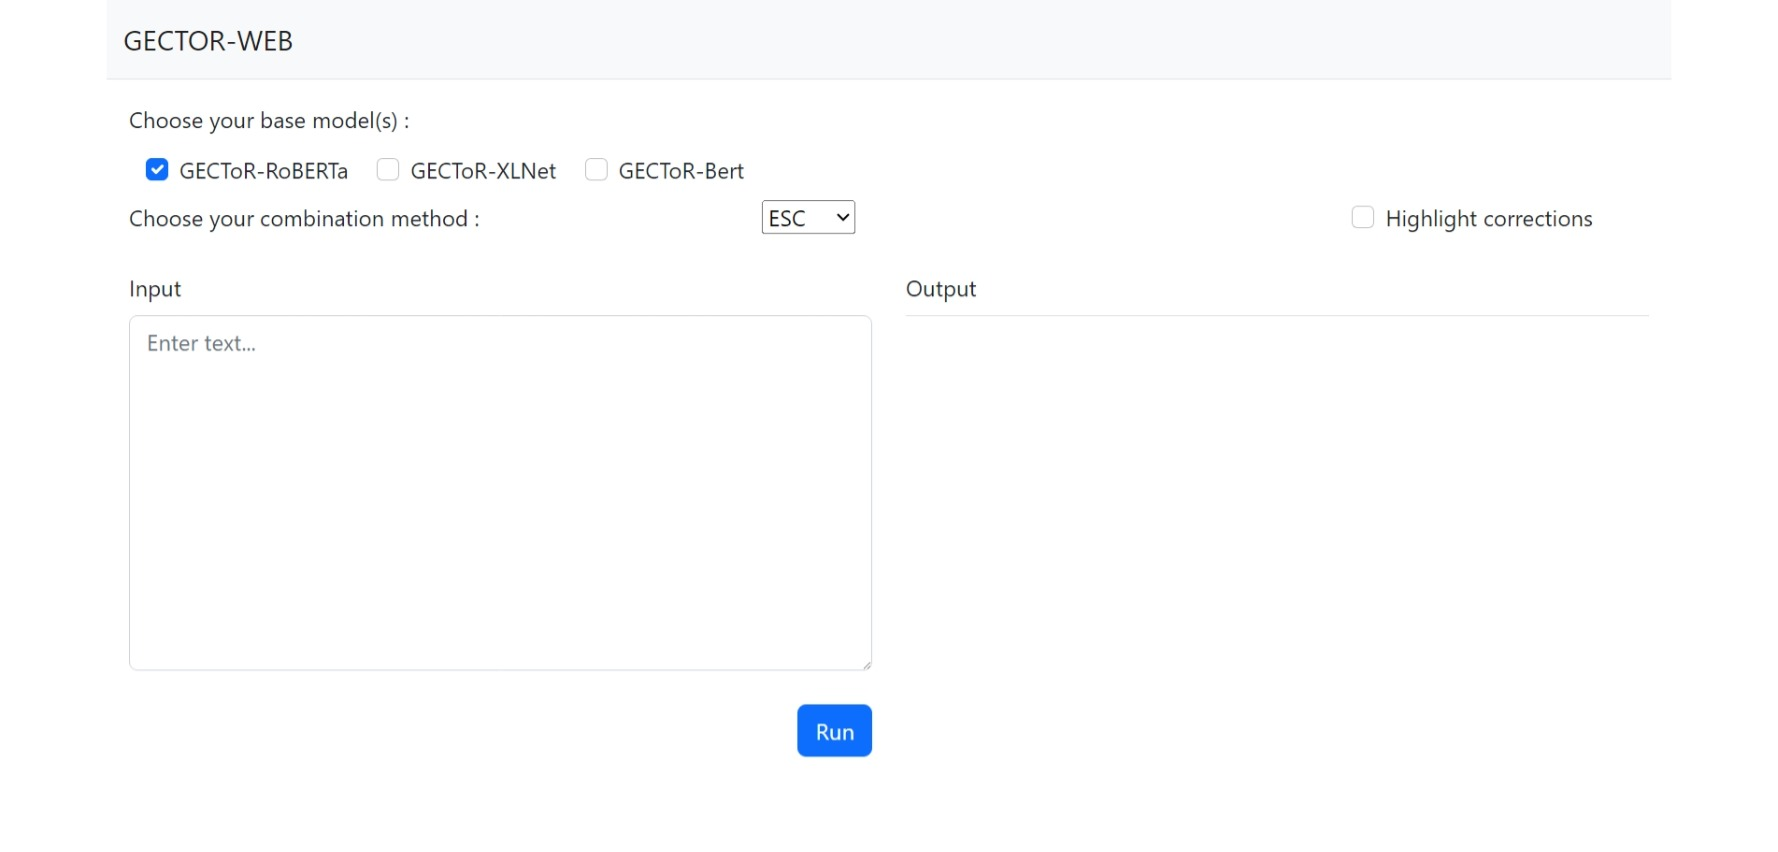
\includegraphics[width=0.85\textwidth]{home}}
      \pause
      \annotatedFigureBox{0.0905,0.7727}{0.4305,0.8393}{i}{0.4305,0.8393}%tr
      \pause
      \annotatedFigureBox{0.434,0.7266}{0.5105,0.8003}{ii}{0.5105,0.8003}%tr
      \pause
      \annotatedFigureBox{0.7615,0.7308}{0.9195,0.7934}{iii}{0.9195,0.7934}%tr
      \pause
      \annotatedFigureBox{0.1285,0.3489}{0.4595,0.6243}{iv}{0.4595,0.6243}%tr
      \pause
      \annotatedFigureBox{0.574,0.2591}{0.8665,0.6118}{v}{0.8665,0.6118}%tr
    \end{annotatedFigure}
    \caption{The User Interface of GecWeb.}
  \end{figure}

  \note<1>{The interface of GecWeb consists of five components, which are:}
  \note<2>{base model selection}
  \note<3>{combination method selection}
  \note<4>{output mode}
  \note<5>{input text box}
  \note<6>{output text box}
\end{frame}

\subsection{GecWeb Demo}

\begin{frame}{GecWeb Demo (Browser)}
  \begin{figure}
    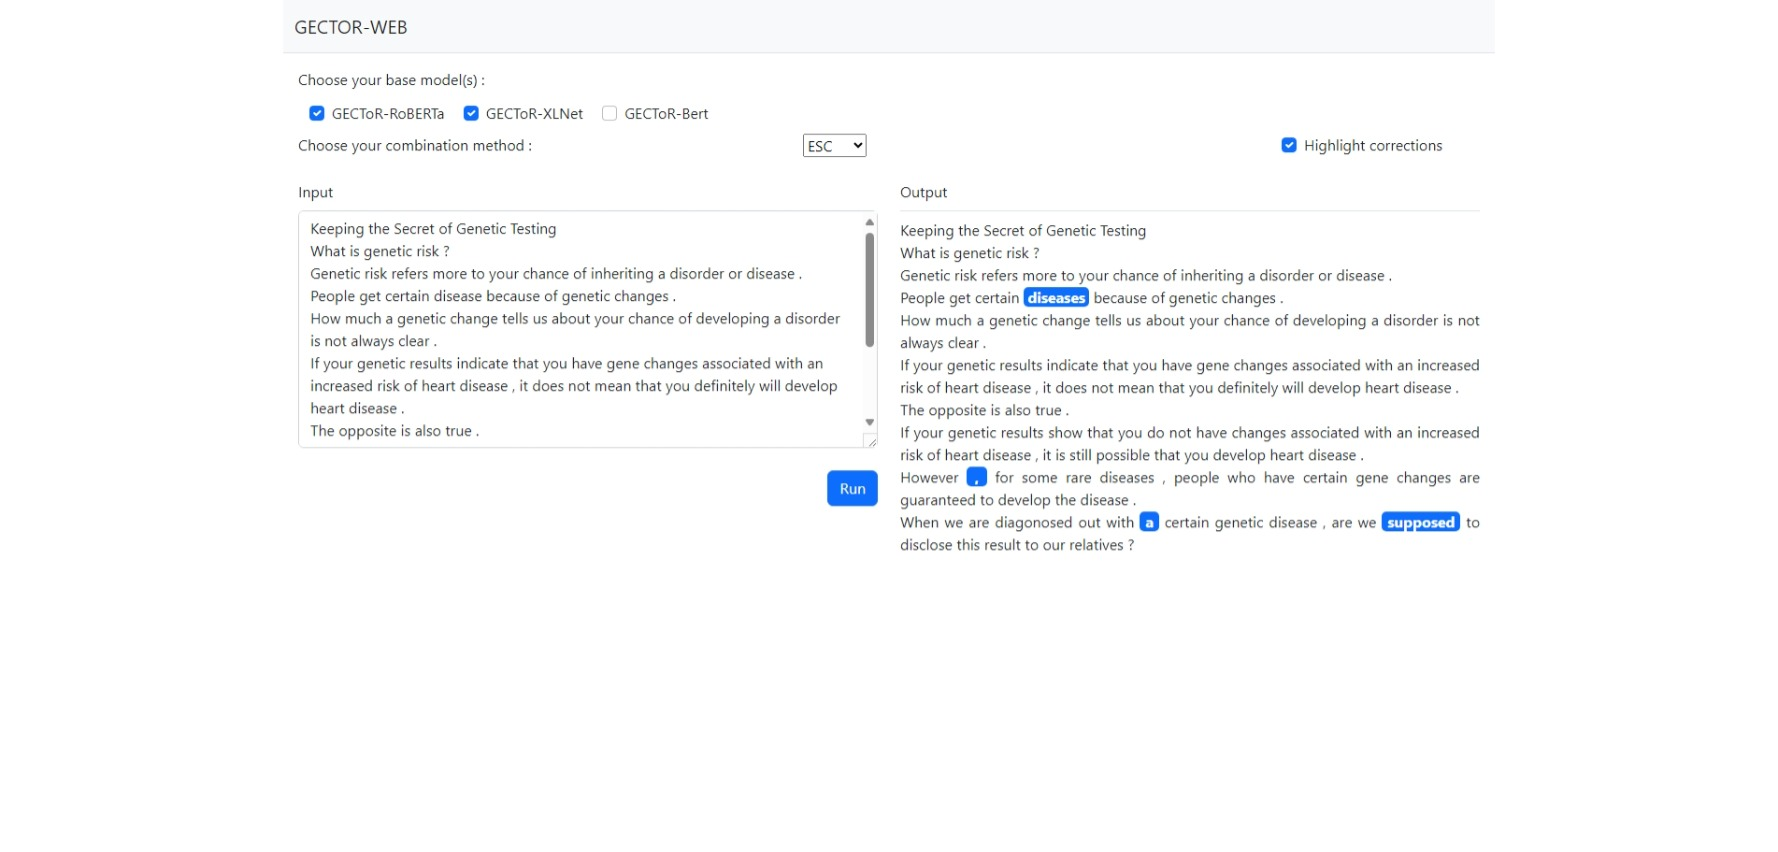
\includegraphics[width=0.9\textwidth]{highlight}
    \caption{GecWeb running on a browser.}
  \end{figure}
\end{frame}

\begin{frame}{GecWeb Demo (Browser)}
  \begin{figure}
    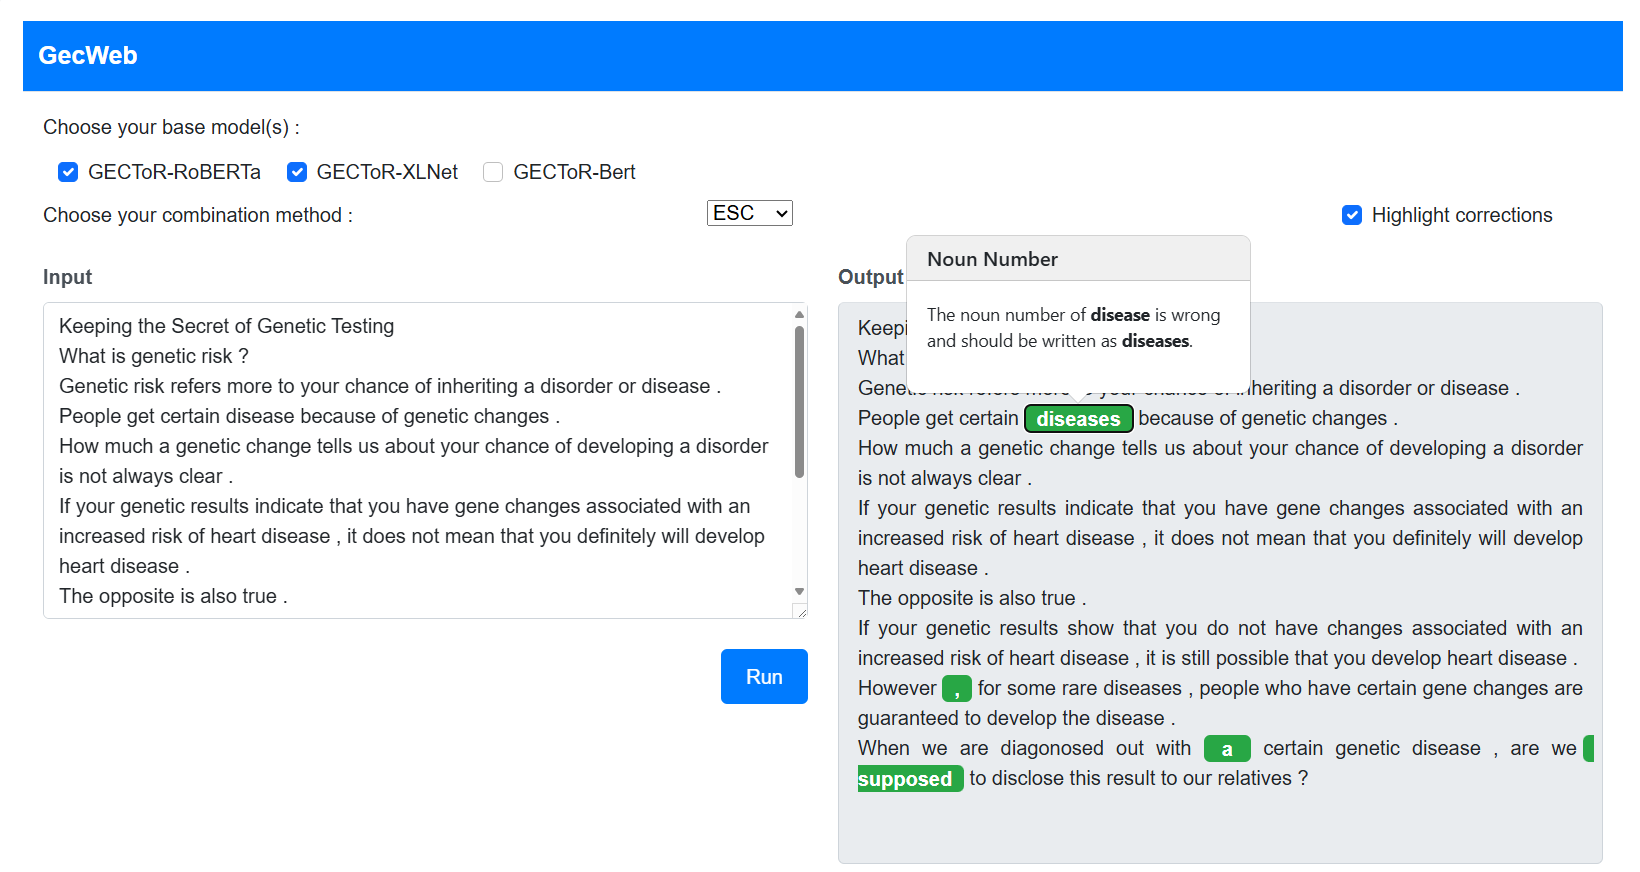
\includegraphics[width=0.8\textwidth]{highlight+note}
    \caption{GecWeb running on a browser.}
  \end{figure}
\end{frame}

\begin{frame}{GecWeb Demo (Mobile)}
  \begin{figure}
    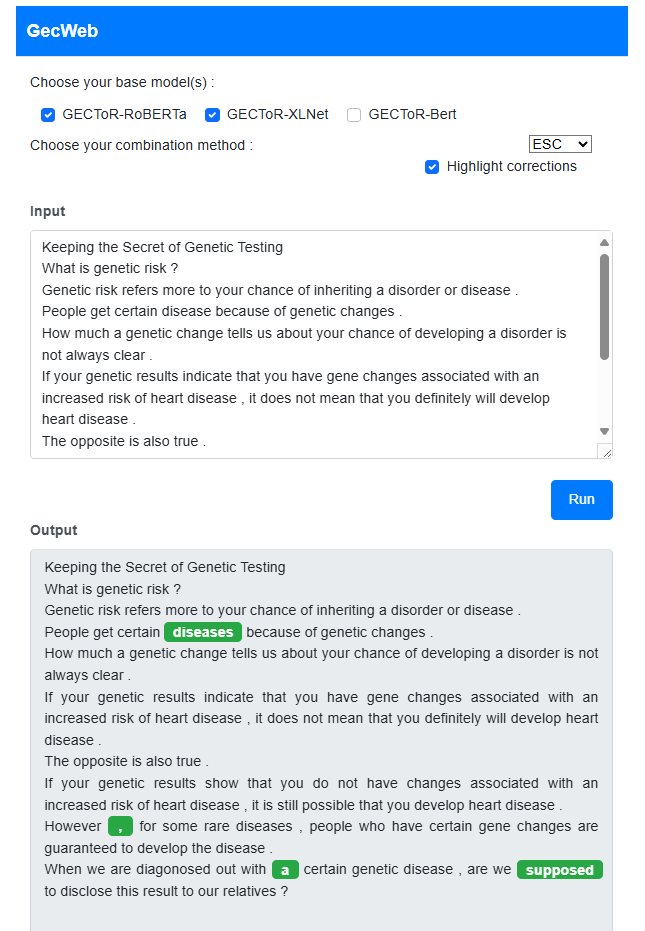
\includegraphics[height=0.75\textheight]{mobile}
    \caption{GecWeb running on a mobile phone.}
  \end{figure}
\end{frame}
